\section{Raw tikzpicture with override}

\begin{figure}
\begin{center}
    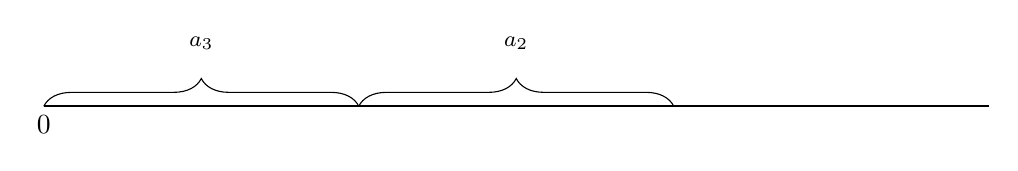
\begin{tikzpicture}[scale=1]
      \draw[thick] (0,0) -- (12,0);
      \node at (0,0) [below] {$0$};
      \draw [decorate,decoration={brace,amplitude=10pt}]
        (0,0) -- (4,0) node [black,midway,yshift=0.8cm] {\footnotesize $a_3$};
      \draw [decorate,decoration={brace,amplitude=10pt}]
        (4,0) -- (8,0) node [black,midway,yshift=0.8cm] {\footnotesize $a_2$};
    \end{tikzpicture}
    \caption{\label{f:coase_no} Notation, following \citep{coase1937nature}.}
\end{center}
\end{figure}
